%% LaTeX-Beamer template for KIT design
%% by Erik Burger, Christian Hammer
%% title picture by Klaus Krogmann
%%
%% version 2.1
%%
%% mostly compatible to KIT corporate design v2.0
%% http://intranet.kit.edu/gestaltungsrichtlinien.php
%%
%% Problems, bugs and comments to
%% burger@kit.edu

\documentclass[18pt]{beamer}
\usepackage[utf8x]{inputenc}
\usepackage{units}
\usepackage{booktabs}

%% CUSTOM
\usepackage{amsmath}
\usepackage{algpseudocode}

%% Definitions
\DeclareMathOperator{\div2}{div}
\renewcommand{\algorithmicrequire}{\textbf{Input:}}
\renewcommand{\algorithmicensure}{\textbf{Output:}}
\algnewcommand\algorithmicto{\textbf{to}}
\algrenewtext{For}[3]{\algorithmicfor\ $#1 \gets #2$ \algorithmicto\ $#3$ \algorithmicdo}
\algnewcommand\algorithmicod{\textbf{od}}
\algrenewtext{EndWhile}{\algorithmicod}
\algrenewtext{EndFor}{\algorithmicod}
%\AtBeginSection[]{%
%\begin{frame}<beamer> % do nothing in handouts
%    \frametitle{Überblick}
%    \tableofcontents[sectionstyle=show/shaded,
%    subsectionstyle=show/show/hide]
%\end{frame}
%}
%\AtBeginSubsection[]{%
%\begin{frame}<beamer> % do nothing in handouts
%    \frametitle{Überblick}
%    \tableofcontents[sectionstyle=show/shaded,
%    subsectionstyle=show/shaded/hide]
%\end{frame}
%}

%% SLIDE FORMAT

% use 'beamerthemekit' for standard 4:3 ratio
% for widescreen slides (16:9), use 'beamerthemekitwide'

\usepackage{templates/beamerthemekit}
%\usepackage{templates/beamerthemekitwide}

 %% TITLE PICTURE

 % if a custom picture is to be used on the title page, copy it into the 'logos'
 % directory, in the line below, replace 'mypicture' with the 
 % filename (without extension) and uncomment the following line
 % (picture proportions: 63 : 20 for standard, 169 : 40 for wide
 % *.eps format if you use latex+dvips+ps2pdf, 
 % *.jpg/*.png/*.pdf if you use pdflatex)


 \titleimage{banner}
 
 
%% Define some colors:
\definecolor{darkblue}{rgb}{0,0,.5}
\definecolor{darkgreen}{rgb}{0,.5,0}

 %% TITLE LOGO

 % for a custom logo on the front page, copy your file into the 'logos'
 % directory, insert the filename in the line below and uncomment it

\titlelogo{logo_150x150}
 
 % (*.eps format if you use latex+dvips+ps2pdf,
 % *.jpg/*.png/*.pdf if you use pdflatex)
 
 %% TikZ INTEGRATION
 
 % use these packages for PCM symbols and UML classes
 % \usepackage{templates/tikzkit}
 % \usepackage{templates/tikzuml}
 
 % the presentation starts here
 
\author{Dominik Muth - dominik.muth@student.kit.edu}
\institute{Institut f\"ur Informatik}

\subtitle{Foliensatz 13}
\date{31. Januar 2013}

\newcommand{\sq}{$\square$}
\newcommand{\da}{$\downarrow$}

\begin{document}

\begin{frame}
    \titlepage
\end{frame}

\begin{frame}{Outline/Gliederung}
    \tableofcontents
\end{frame}

\section{Wiederholung}
\begin{frame}{Wiederholung}
    \begin{itemize}
        \item Irgendwas zu Turingmaschinen
        \item Irgendwas zu Codierungen
        \item Irgendwas zu Relationen
        \item Reflexiv
        \item Transitiv
        \item Symmetrisch
    \end{itemize}
\end{frame}
\section{Unentscheidbare Probleme}
\begin{frame}{Unentscheidbare Probleme}
    Es gibt Probleme, die lassen sich mit einer Turing-Maschine (oder äquivalent: einem Java-Programm) nicht lösen. (Auch nicht mit unendlich viel Zeit und Platz.)\\
    Ein solches Problem ist nicht \emph{entscheidbar}
    \begin{block}{Entscheidbarkeit}
        Für ein entscheidbares Problem gibt es eine Turingmaschine, die für jede Eingabe hält und das Eingabewort entweder akzeptiert oder nicht.
    \end{block}
\end{frame}
\begin{frame}{Codierung von Turingmaschinen}
   Bisher haben wir eine Turingmaschine formal so geschrieben $T = \left( Z, Z_0, X, f, g, m \right)$. Wir bauen uns eine Codierung, die die ganze Turingmaschine in ein Wort $w_1$ ``packt''. \\
   Dieses Wort $w_1$ übergeben wir dann einer universellen Turingmaschine $U$, die 
   \begin{itemize}
       \item übeprüft, ob $w_1$ eine Turingmaschine $T$ codiert
       \item dann die Turingmaschine $T$ ``simuliert'' und als Eingabe $w_2$ verwendet
       \item und schließlich das Ergebnis davon ausgibt
   \end{itemize}
   \begin{figure}[h]
       \centering
       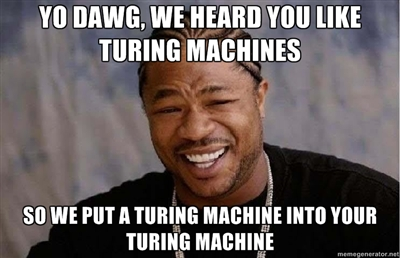
\includegraphics[scale=.5]{graphics/13/33928220.jpg}
   \end{figure}
\end{frame}
\begin{frame}{Halteproblem}
    \begin{block}{Satz}
        Es ist nicht möglich, eine Turingmaschine $U$ zu bauen, die für jede Turingmaschine $T$ (codiert als $w_1$) und jede Eingabe $w_2$  entscheidet, ob $T$ bei der Eingabe von $w_2$ hält.
    \end{block}
    Das lässt sich auch beweisen. 
    Halteproblembeweis (verdorbene Diagonale)
\end{frame}
\section{Äquivalenzrelationen}
\begin{frame}{Äquivalenzrelation}
    \begin{block}{Definition: Äquivalenzrelation}
        Eine Relation $R$ ist genau dann eine \emph{Äquivalenzrelation}, wenn sie
        \begin{itemize}
            \item symmetrisch,
            \item reflexiv und
            \item transitiv
        \end{itemize} ist.
    \end{block}
\end{frame}
\begin{frame}{Eigenschaften von Relationen}
    Welche Eigenschaften haben diese Relationen (stets auf ganze Zahlen)?
    \begin{itemize}
        \item $\leq$ \visible<2->{reflexiv, transitiv}
        \item $>$ \visible<3->{transitiv}
        \item $=$ \visible<4->{reflexiv, transitiv, symmetrisch}
    \end{itemize}
    Wie sieht das in einem Graphen aus? (Tafel)
\end{frame}
\begin{frame}{Äquivalenzklasse}
    \begin{block}{Definition: Äquivalenzklasse}
        Sind zwei Elemente $\left( x,y \right)\in R$, so schreibt man auch $xRy$ (Infixschreibweise). Alle Elemente, die miteinander in Relation stehen, befinden sich in der selben \emph{Äquivalenzklasse}:
        \begin{align*}
            [x]_\mathrm{R} = \left\{ y | yRx \right\}
        \end{align*}
    \end{block}
\end{frame}
\begin{frame}{Quiz}
    \begin{itemize}
        \item Stimmt es, dass auch $xRy$ folgt: $[x]_\mathrm{R} = [y]_{\mathrm{R}}$? \visible<2->{Ja.}
        \item Existiert ein $z\in \left[ x \right]_\mathrm{R}$ und $z\in\left[ y \right]_\mathrm{R}$, so ist $\left[ x \right]_\mathrm{R} = \left[ y \right]_\mathrm{R}$. \visible<3->{Ja.}
        \item Wieviele Äquivalenzklassen gibt es zu $R = \mod 6$? \visible<4->{6}
    \end{itemize}
\end{frame}
\begin{frame}{Nerode-Äquivalenzrelation}
    \begin{block}{Definition: Nerode-Äquivalenzrelation}
        Sei $L\subseteq A^*$ eine formale Sprache. $w_1$ und $w_2$ seien Wörter $\in A^*$. Die Wörter heißen \emph{Nerode-Äquivalent} ($\equiv_L$), falls gilt:
        \begin{align*}
            w_1 \equiv_L w_2 \leftrightarrow \left( \forall w \in A^*: w_1 w\in L \leftrightarrow w_2 w\in L \right)
        \end{align*}
    \end{block}
\end{frame}
\begin{frame}{Beispiel zur Nerode Äquivalenz}
    \begin{itemize}
        \item Alphabet $A = \left\{ a,b \right\}$
        \item Sprache $L \subset A*$, $L$ enthält alle Wörter ohne das Teilwort $ba$: $L = \left< a^* b^*\right>$
    \end{itemize}
    Wie sieht der zugehörige Automat aus?
    \begin{columns}
        \begin{column}{.5\textwidth}
            \visible<2->{\begin{figure}
                \centering
                \begin{tikzpicture}[shorten >=1pt,initial text=,node distance=2cm,auto,->,>=stealth]
                    \node[state,initial,accepting]  (1)                    {1};
                    \node[state,accepting]  (2)[right of=1]        {2};
                    \node[state]  (J)[below right of=1]  {J};

                    \path[->]
                        (1) edge              node  {b} (2)
                        (1) edge [loop above] node  {a} ()
                        (2) edge [loop above] node  {b} ()
                        (2) edge              node  {a} (J)
                        (J) edge [loop below] node  {a,b} ()
                    ;
                \end{tikzpicture}
            \end{figure}}
        \end{column}
        \begin{column}{.5\textwidth}
            \visible<3->{Wie kann jeder Zustand erreicht werden?}
            \visible<4->{\begin{itemize}
                \item $a^*$
                \item $a^*bb^*$
                \item $a^*bb^*a\left\{ a,b \right\}^*$
            \end{itemize}}
            Nerode-Äquivalenzklassen: $\visible<5->{\left[ \epsilon \right], \left[ b \right], \left[ ba \right]$.}
        \end{column}
    \end{columns}
\end{frame}
\begin{frame}{Faktormenge}
    \begin{block}{Definition: Faktormenge}
        Die Menge aller Äquivalenzklassen einer Menge zur Relation $R$ bezeichnet man als \emph{Faktormenge} und schreibt $M_\mathrm{/R}$.
    \end{block}
\end{frame}
\begin{frame}{Beispiel 2 zur Nerode-Äquivalenz}
    Gegeben sei die Sprache $L = \left\{ a^k b^k | k \in \mathbb{N}_0 \right\}$. \\
    Wie sieht hier ein endlicher Akzeptor aus?
    \visible<2->{Es gibt keinen.}\\
    \visible<3->{Nennt einige Nerode-Äquivalenzklassen.}\\
    \visible<4->{Wieviele gibt es?}\\
    \visible<5->{Es gibt unendlich viele Nerode-Äquivalenzklassen. Die Faktormenge hat also unendlich viele Elemente.}
\end{frame}
\end{document}
